\chapter{Methodology}\label{ch:metodologia}

In the following sections, the methodology for data generation, managment and analysis will be presented. To adress these issues, we will use Python \cite{McKinney,VanderPlas} due to 
its versatility and the wide range of libraries available. The two used will be NumPy \cite{numpy} and Matplotlib \cite{matplotlib} for the visualization.
 
\section{Time series factory}\label{sec:time_series_factory}

The first step is the generation of time series, there are two ways to do this: the slow one and the fast one. The first one is discretizing the time and calculating the rate at each time step
according with Eq \ref{eq: Hawkes rate}, then accept or reject the event if $p<\lambda \cdot dt$ for a random number $p\in \mathcal{U}[0,1]$ . 
This method works for small time series, but for large ones is not efficient because the summation of the kernel function has to be done at each time step. The pseudo-code for this method is
presented in Algorithm \ref{alg: slow method}.

\begin{algorithm}
    \caption{Slow method to generate Hawkes processes.}\label{alg: slow method}
    \begin{algorithmic}
        \Require $t_max$, $n_{intervals}$, $\lambda(t_0)=\mu$, $p$
        \State $dt \gets \frac{t_{max}}{n_{intervals}}$
        \For {$i=0$ to $n_{intervals}$}1
            \State $\lambda(t_k) \gets \mu + n\sum_{t_i<t_k}\phi(t_k-t_i)$ \Comment{$t_i=i\cdot dt$}
            \If {$\lambda(t_k)\cdot dt > p$}
                \State $t_{event} \gets t_k$
            \EndIf
        \EndFor
        \end{algorithmic}
\end{algorithm}

The fast method takes advantage of Monte Carlo methods \cite{barbu2020monte} to generate the time series. The idea of this procedure consists in computing the inter-event time instead 
of the time of the event. To get to the algorithm, we start from the following expression:

\begin{equation}
    PDF(\text{inter-event time}=\Delta t) = \lambda(t+\Delta t) e^{-\int_t^{t+\Delta t}\lambda(t^\prime)dt^\prime} 
    \label{eq: inter-event time PDF}
\end{equation}

To demonstrate this, we have to take a look at the Figure \ref{f: Figura calculo probabilidad acumulada} and recall that $\lambda$ is a probability per unit of time.

\begin{figure}[H]
    \centering
    \includegraphics[width=0.7\textwidth]{Figura cálculo probabilidad acumulada.png}
    \caption{Diagram to calculate the cumulative probability of the inter-event time.}
    \label{f: Figura calculo probabilidad acumulada}
\end{figure}

The probability per unit of time of having an event in the interval $[t+\Delta t,t+\Delta t+dt]$ is the probability of no events in the interval $[t,t+\Delta t]$ times the probability 
of happening in the interval $[t+\Delta t,t+\Delta t+ dt]$. Putting words into mathematics, we have that the probability of not having an event in the interval $[t,t+\Delta t]$ is:
\begin{equation}
    \begin{split}
        P(\text{event}\in [t+\Delta t+dt])=& \left(1-\lambda(0)\cdot dt \right)\left(1-\lambda(dt)\cdot dt \right)\left(1-\lambda(2dt)\cdot dt \right)\ldots\\
        =& \prod_{k=0}\underbrace{\left(1 -\lambda(k dt)\cdot dt \right)}_{e^{\ln \left(1-\lambda(k dt)dt \right)}}=e^{\sum_{k=0}\ln \left(1-\lambda(k dt) dt \right)}= \ldots\quad \text{Using}  \ln(1-\varepsilon)\approx -\varepsilon\\
        =& e^{-\sum_{k=0}\lambda(kdt)dt}\underbrace{=}_{dt\to 0}e^{-\int_{t}^{t+\Delta t}\lambda(t^\prime)dt^\prime}.
    \end{split}
    \label{eq: probability of no events}
\end{equation} 
Knowing that the probability of having an event in the interval $[t+\Delta t,t+\Delta t+dt]$ is $\lambda(t+\Delta t)dt$, we have:

\begin{equation}
P(\text{event}\in [t+\Delta t,t+\Delta t+dt])\cancel{dt}= \lambda(t+\Delta t)dt\cdot e^{-\int_{t}^{t+\Delta t}\lambda(t^\prime)dt^\prime}\times PDF(\text{inter-event time}=\Delta t)\cancel{dt}.
\label{eq: probability of having an event}
\end{equation}

Having that we can calculate the inter-event time following the next steps. 

$$ \text{PDF}\left( \text{inter-event time } = \Delta,t \right) = \lambda(t+\Delta t)\times \underbrace{e^{\int_{t}^{t+\Delta t}\lambda(t^{\prime}dt^\prime)}}_{\text{No events during }(t,t+\Delta t)}$$

In order to generate $\Delta t$, we will use the inverse transform method \cite{Toral}, therefore we have to calculate the cumulative probability of the inter-event time:
\begin{equation}
    \begin{split}
        \text{accum}(\Delta t)=&\int_{0}^{\Delta t}\text{PDF}\left( \Delta t^\prime \right)d\Delta t^\prime = u\in\mathcal{U}  [0,1]\\
        &\int_{0}^{\Delta t} \underbrace{\lambda(t+\Delta t^\prime)e^{\int_{t}^{t+\Delta t^\prime}\lambda(t^{\prime})dt^{\prime}}}_{-\dfrac{d}{d\Delta t^{\prime}}\left[ e^{-\int_{t}^{t+\Delta t}\lambda t^\prime dt^\prime} \right]}d\Delta t^\prime=u \qquad  \text{Using Barrow rule}\\
        &-e^{-\int_{t}^{t+\Delta t}\lambda(t^\prime)dt^\prime}\Big|_{0}^{\Delta t}=1-e^{-\int_{t}^{t+\Delta t}\lambda(t^\prime)dt^\prime}=u\qquad  \text{Taking logarithms}\\
        &\int_{t}^{t+\Delta t}\lambda(t^\prime)dt^\prime=-\ln(1-u) = \ln (\bar{u})\\
    \end{split}
    \label{eq: cumulative probability}
\end{equation}

To compute the inter-event time, we have to generate $\bar{u}\sim$ and solve the equation. Having in mind this relation and using Eq \ref{eq: Hawkes rate at event time} we have:
EN EL LA ECUACIÓN REFERENCIADA Y LA SEGUNDA EXPONENCIAL SE PUEDE PONER $\lambda(t_k^-)$ en lugar de $\lambda(t_k)$? .
\begin{equation}
    \begin{split}
        u=&1-e^{-\mu(t-t_k)}e^{-(\lambda(t_k)+\alpha-\mu)\cdot\overbrace{\int_{t_k}^{t}e^{-\beta(t^\prime)-t_k}dt^\prime}^{-\frac{1}{\beta}\left[ e^{-\beta}(t-t_k)-1 \right]}}\\
        u=&1-\underbrace{e^{-\mu(t-t_k)}}_{P(t_{k+1}^{(1)}>t)}\underbrace{e^{-\left[ (\lambda(t_k)+\alpha-\mu)\beta^{-1}\left( 1-e^{-\beta(t-t_k)} \right) \right]}}_{{P(t_{k+1}^{(2)}>t)}}
    \end{split}
    \label{eq: u = 1 - P(t_{k+1} > t)P(t_{k+1} > t), previo al composition method}
\end{equation}

Then we apply the composition method \cite{dassios2013exact}. If we take $t_{k+1}=\min(t_{k+1}^(1),t_{k+1}^(2))$; then $t_{k+1}\sim P(t_{k+1}>t)$, hence:
\begin{equation}
    \begin{split}
        \text{Prob}(t_{k+1}=\min\left(  t_{k+1}^{(1)},t_{k+1}^{(2)} \right)\leq t)=&1-\text{Prob}\left( \min \left( t_{k+1}^{(1)},t_{k+1}^{(2)}\right)>t \right)\\
        =&1-\text{Prob}\left( t_{k+1}^{(1)}>t \right)\cdot\text{Prob}\left( t_{k+1}^{(2)}>t \right)\\
    \end{split}
    \label{eq: composition method}
\end{equation}
where we have used that the probability that the smaller is greater than $t$ is that each separately is greater than $t$ because both have to be greater than $t$. As we can 
see the expressions in Eqs \ref{eq: u = 1 - P(t_{k+1} > t)P(t_{k+1} > t), previo al composition method} and \ref{eq: composition method} are the same, so we can use the composition 
method to generate the inter-event time. Then, the algorithm to generate the inter-event time is:
\begin{enumerate}
    \item Generate $t_{k+1}^{(1)}\sim P \left( t_{k+1}^{(1)}>t \right) = e^{-\mu\left( t-t_k \right)}$ using 
    $$P\left( t_{k+1}^{(1)}\leq t \right) = \underbrace{1- \underbrace{e^{-\mu(t-t_k)}}_{\bar{u_1}\in\mathcal{U}[0,1]}}_{1-\bar{u_1}=u_1}=u_1 \in \mathcal{U}[0,1]$$
    This is done by generating $u_1\in\mathcal{U}[0,1]$ and solving the equation.
    \begin{equation}
        \begin{split}
        &u_1=1-e^{-\mu\left( t_{k+1}^{(1)}-t_k \right)}\\
        &\ln(u_1)=-\mu\left( t_{k+1}^{(1)}-t_k  \right)\Rightarrow t_{k+1}^{(1)}=t_k-\dfrac{\ln(u_1)}{\mu}            
        \end{split}
        \label{eq: inter-event time 1}
    \end{equation}
    \item Generate $t_{k+1}^{(2)}\sim P\left( t_{k+1}^{(2)}>t \right)=e^{-\left( \left( \lambda(t_k)+\alpha-\mu \right)\beta^{-1}\left( 1-e^{-\beta\left( t_{k+1}^{(2)-t_k}\right)}\right)\right)}$
    in a similar way as before:
    \begin{equation}
        \begin{split}
            &u_2=1-e^{-\left( \left( \lambda(t_k)+\alpha-\mu \right)\beta^{-1}\left( 1-e^{-\beta\left( t_{k+1}^{(2)-t_k}\right)}\right)\right)}\\
            -&\ln(u_2)=\left( \left( \lambda(t_k)+\alpha-\mu \right)\beta^{-1}\left( 1-e^{-\beta\left( t_{k+1}^{(2)-t_k}\right)}\right)\right)\\ 
            & 1+\dfrac{\beta\ln u_2}{\lambda(t_k)+\alpha-\mu}=e^{-\beta\left( t_{k+1}^{(2)-t_k}\right)}\\
            &t_{k+1}^{(2)}=t_k-\beta^{-1}\ln\underbrace{\left( 1+\dfrac{\beta\ln u_2}{\lambda(t_k)+\alpha-\mu} \right)}_{\text{This number must be positive}}   
        \end{split}
        \label{eq: inter-event time 2}
    \end{equation}   
    \item Choose $t_{k+1}=\min\left( t_{k+1}^{(1)},t_{k+1}^{(2)} \right)$
    \item Calculate the rate at $t_{k+1}$ using Eq \ref{eq: Hawkes rate exponential becomes Markovian} and go back to step 1.
\end{enumerate}

With this method, we can generate time series efficiently. The pseudo-code for this method is presented in Algorithm \ref{alg: fast method}.
\begin{algorithm}
    \caption{Algorithm to generate $K$ Hawkes events.}\label{alg: fast method}
    \begin{algorithmic}
        \Require $\alpha$, $\beta$, $\lambda(t_0)=\mu$, $K$
        \For {$k=0$ to $K$}
            \State $u_1,u_2 \gets \mathcal{U}[0,1]$
            \State $t_{k+1}^{(1)}\gets \dfrac{\ln(u_1)}{\mu}$
            \State $t_{k+1}^{(2)} \gets \beta^{-1}\ln\left( 1+\dfrac{\beta\ln u_2}{\lambda(t_k)+\alpha-\mu} \right)$
            \State $t_{k+1} \gets \min\left( t_{k+1}^{(1)},t_{k+1}^{(2)} \right)$
            \State $\lambda(t_{k+1}) \gets \mu + e^{-\beta(t_{k+1}-t_k)}\left( \lambda(t_k)-\mu+n \right)$
        \EndFor
    \end{algorithmic}
\end{algorithm}

To conclude generation of time series section, we can generalise the algorithm in order to generate $M$ Hawkes processes coupled \cite{dassios2013exact,laub2021elements}. 
In this work we will generate 2 coupled Hawkes processes, one corresponding to an excitatory population and the other to an inhibitory population. The essence of the algorithm is the 
same as the one presented. First, we generate the inter-event time for the excitatory population and the inhibitory population, after that, we choose the minimum of both and update the
rates of both populations according to the event that has just occurred. Mathematically it is expressed as follows:

\begin{enumerate}
    \item Generate $\Delta_{k+1} = \min\left\{ \Delta_{k+1}^{(1)},\Delta_{k+1}^{(2)} \right\}$ with $\Delta_{k+1}^{(j)}=t_{k+1}^{(j)}-t_k^{(j)}$ generated 
    as in Eqs \ref{eq: inter-event time 1} and \ref{eq: inter-event time 2}.
    \begin{equation}
        \Delta_{k+1}^{(j)} = \min \left\{ -\dfrac{\ln(u_1^{(j)})}{\mu_j},-\beta_j^{-1}\ln\left( \underbrace{1+\dfrac{\beta_j\ln u_2^{(j)}}{\lambda_j\left( t_k^{(j)} \right)+\alpha_j-\mu_j}}_{g_j} \right) \right\}
        \label{eq: inter-event time coupled}
    \end{equation}
    Note that $g_j$ must be positive, otherwise, take the other term.
    \item Once we have the process $(l)$, we update the time for the following event as $t_{k+1}=t_k+\Delta_{k+1}^{(l)}$.
    \item Update the rates for the excitatory and inhibitory populations as follows:
    \begin{equation}
        \lambda_j(t_{k+1}) = \mu_j + e^{-\beta_j(t_{k+1}-t_k)}\left( \lambda_j(t_k)-\mu_j+\alpha_{l\to j} \right) \qquad \text{with } j=1,2
    \end{equation}
\end{enumerate}

The pseudo-code for this method is presented in Algorithm \ref{alg: fast method coupled}.

\begin{algorithm}
    \caption{Algorithm to generate $K$ Hawkes events for two coupled processes.}\label{alg: fast method coupled}
    \begin{algorithmic}
        \Require $\alpha_{11}$, $\alpha_{12}$, $\beta_1$, $\mu_1$, $\alpha_{22}$, $\alpha_{21}$, $\beta_2$, $\mu_2$, $K$
        \For {$k=0$ to $K$}
            \State $u_1^{(1)},u_2^{(1)},u_1^{(2)},u_2^{(2)} \gets \mathcal{U}[0,1]$
            \State $\Delta_{k+1}^{(1)}\gets \min\left( -\dfrac{\ln(u_1^{(1)})}{\mu_1},-\beta_1^{-1}\ln\left( 1+\dfrac{\beta_1\ln u_2^{(1)}}{\lambda_1(t_k)+\alpha_{11}-\mu_1} \right) \right)$
            \State $\Delta_{k+1}^{(2)}\gets \min\left( -\dfrac{\ln(u_1^{(2)})}{\mu_2},-\beta_2^{-1}\ln\left( 1+\dfrac{\beta_2\ln u_2^{(2)}}{\lambda_2(t_k)+\alpha_{22}-\mu_2} \right) \right)$
            \State $l\gets \arg\min\left( \Delta_{k+1}^{(1)},\Delta_{k+1}^{(2)} \right)$
            \State $t_{k+1}\gets t_k+\Delta_{k+1}^{(l)}$
            \State $\lambda_1(t_{k+1}) \gets \mu_1 + e^{-\beta_1(t_{k+1}-t_k)}\left( \lambda_1(t_k)-\mu_1+\alpha_{l\to 1} \right)$
            \State $\lambda_2(t_{k+1}) \gets \mu_2 + e^{-\beta_2(t_{k+1}-t_k)}\left( \lambda_2(t_k)-\mu_2+\alpha_{l\to 2} \right)$
        \EndFor
    \end{algorithmic}
\end{algorithm}

\section{When physics and cooking merge}\label{sec:physics_cooking}

Once we have a method to generate time series, we can start analyzing them. We should stablish a control parameter to distinguish between different regimes of the process. In this case,
we will define resolution parameter $\Delta >0$ as a time interval which will help us to identify clusters of activities. Our time series will have $K$ events that occur in times 
$\left\{ t_1,\ldots, t_K \right\}$. Considering this, a cluster os events starts at time $t_i$ and ends at time $t_j$ if $t_j-t_i\leq \Delta$. The number of events in the cluster (cluster 
size) is the number of events in the interval $[t_i,t_j]$ and it's duration is $t_j-t_i$. The extreme cases are when $\Delta$ is smaller than the minimun inter-event time, in this case,
each event is a cluster of size 1 and duration 0. On the other hand when $\Delta$ is greater than the largest inter-event time, all the events are in the same cluster of size $K$ and
duration $t_K-t_1$. Between these two extremes, we will have different regimes of the process and we should be careful with the choice of $\Delta$ because it will determine the
characteristics of the clusters and their statistics. To identify these regimes, we need a phase diagram, in our case, it will be a percolation 
diagram where we will plot the percolation strength $P_{\infty}$ as a function of the resolution parameter $\Delta$. The percolation strength is defined as the fraction of events that are
in the largest cluster over the total number of events. Three different set of parameters will be used to generate the time series in order to compare them. The parameters $\alpha$ and 
$\beta$ will be fixed to 1 in all cases, the other parameters are shown in Table \ref{tab: parameters}.

\begin{table}[H]
    \centering
    \caption{Configuration of the parameters for the simulations}
    \label{tab: parameters}
    \begin{tabular}{@{}lcc@{}}
    \toprule
    Configuration & \multicolumn{1}{c}{$\mu$} & \multicolumn{1}{c}{$n$} \\ \midrule
    First & 1 & 0 \\
    Second & $10^{-4}$ & 1 \\
    Third & $10^2$ & 1 \\ \bottomrule
    \end{tabular}
\end{table}

The percolation diagram will be generated by generating 1000 time series for each configuration and calculating the percolation strength for each one because in general they are not stationary
processes as we can observe in Figure \ref{f: Hawkes not stationary}.

\begin{figure}[H]
    \centering
    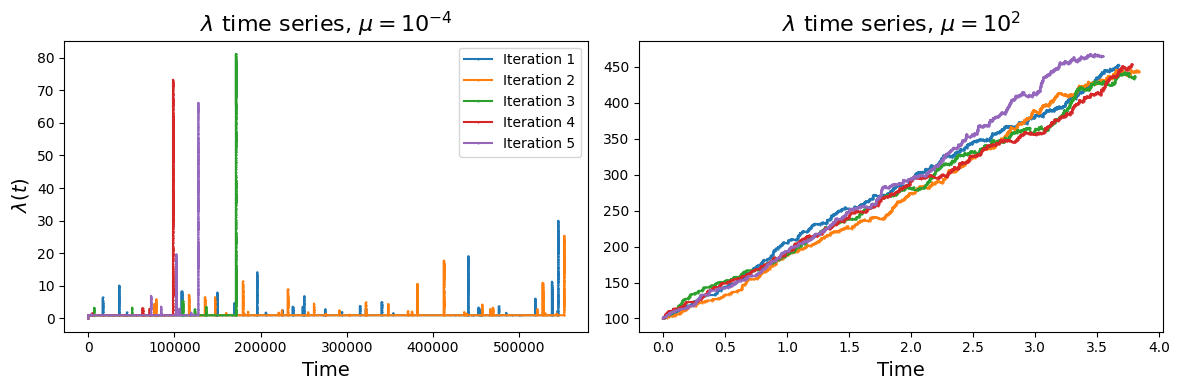
\includegraphics[width=0.9\textwidth]{Signals.png}
    \caption{Five a temporal series of $K=10^5$ events of Hawkes processes with $\mu=10^{-4}$ on the left side and $\mu = 10^2$ on the right one.}
    \label{f: Hawkes not stationary}
\end{figure}

Beginning with the first configuration, we have an homogeneous Poisson process which we know that its interevent time will be distributed randomly with a probability of having an inter-event
time $x_i$ given by $P(x_i)=\mu e^{-\mu x_i}$. Consequently, two consecutive events will be a part of a cluster fixing the resolution parameter to $\Delta$ with a probability of
\begin{equation}
    P(x_i\leq \Delta)=1-e^{-\mu\Delta}\quad\quad \forall i.
    \label{eq: Poisson prob of cluster of size 2}
\end{equation}

This represents the probability in a homogeneous 1D percolation model \cite{stauffer2018introduction}, where we can identify a non percolant phase and a percolant phase separated by the
critical point $\Delta^*$. We can calculate this parameter if we know the maximum inter-event time of the time series. Let us assume that our time series has $K$ events, therefore, it will 
percolate if the condition we have just stablished is satisfied. We can calculate this threshold as the average of the maximum inter-event time in $K$ samples from the 
inter-event time distribution solving the following equation:
\begin{equation}
    \begin{split}
        &K\int_{\Delta^*}^{\infty}P(x) dx=1\\
        &K\int_{\Delta^*}^{\infty}\mu e^{-\mu x}dx=1\\
        &-K\left[ e^{-\mu x} \right]_{\Delta^*}^{\infty}=K\left[ e^{-\mu\Delta^*} - \cancelto{0}{e^{-\mu\infty}\quad} \right]=1\\
        &K e^{-\mu\Delta^*}=1\\
        &\Delta^*(K)=-\dfrac{\ln\left(K \right)}{\mu}
    \end{split}
    \label{eq: critical point}
\end{equation}

For the other two configurations, on both we have a self-exciting process with $n=0$, which means that we have a critical dynamical regime as we shall see later but with different background 
rates, one much smaller than 1 and the other much greater than 1. This fact will be reflected in the percolation diagram. We will not approach this cases from a theoretical point of view
but from a graphic one. With the second configuration, as we have seen in Figure \ref{f: Hawkes rate burst} if the condition $\mu\ll 1$ is satisfied, we will have a bursty structure in the 
time series. Due to the low background rate, the events are less likely to occur, but when they do, they tend to form avalanches of activity thanks to the self-excitation. This will be
reflected in the percolation diagram as a first phase transition at a critical point $\Delta^*_1$ when $\Delta$ is of the order of the average cluster size. Then, a second phase transition
will occur at a critical point $\Delta^*_2$ when $\Delta$ is greater than the greatest inter-event time. This phenomena is illustrated in Figure \ref{f: Delta percolación}.

\begin{figure}[H]
    \centering
    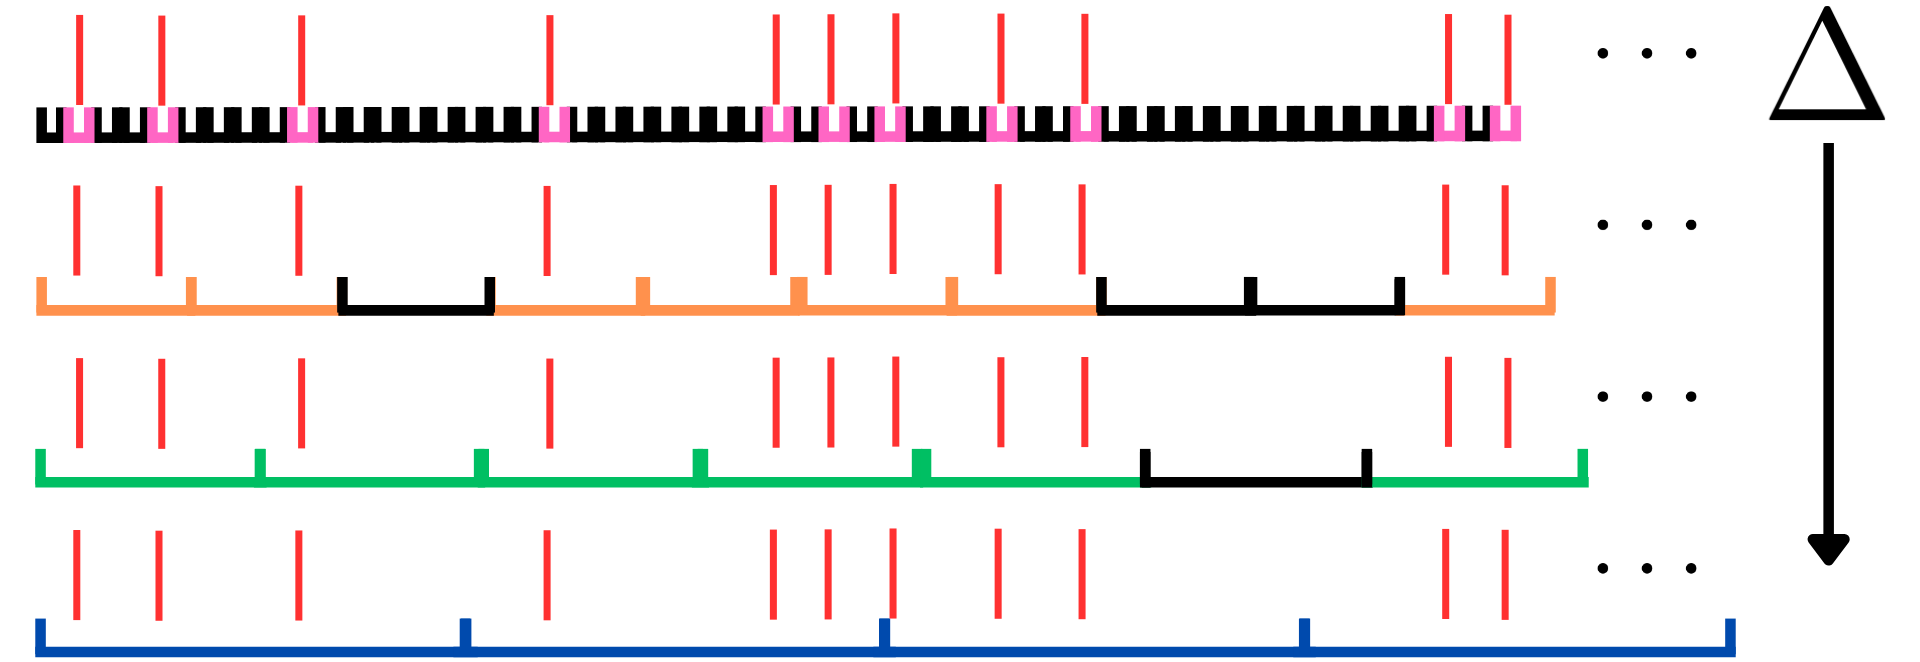
\includegraphics[width=0.9\textwidth]{Raster plot deltas.png}
    \caption{Diagram for $\mu\ll 1$. Red lines represent the events, clusters are coloured. As we can see, we have two regimes, one when $\Delta$ is of the order of the average 
    cluster size and another when is of the order of the inter-event time where the system percolates.}
    \label{f: Delta percolación}
\end{figure}

On the other hand, when $\mu\gg 1$ events occur more frequently, without making the bursty structure of Figure \ref{f: Hawkes rate burst}, but making a more regular structure as
illustrated in Figure \ref{f: Hawkes rate burst 2}. This will be reflected in the phase diagram as a single phase transition at a critical point $\Delta^*$ when $\Delta$ is of the order of
the average cluster size. This phenomena is illustrated in Figure \ref{f: Delta percolación 2}. Note the absence of a time scale in both diagram, they are diagrams for the explanation of 
the phase diagram.

\begin{figure}[H]
    \centering
    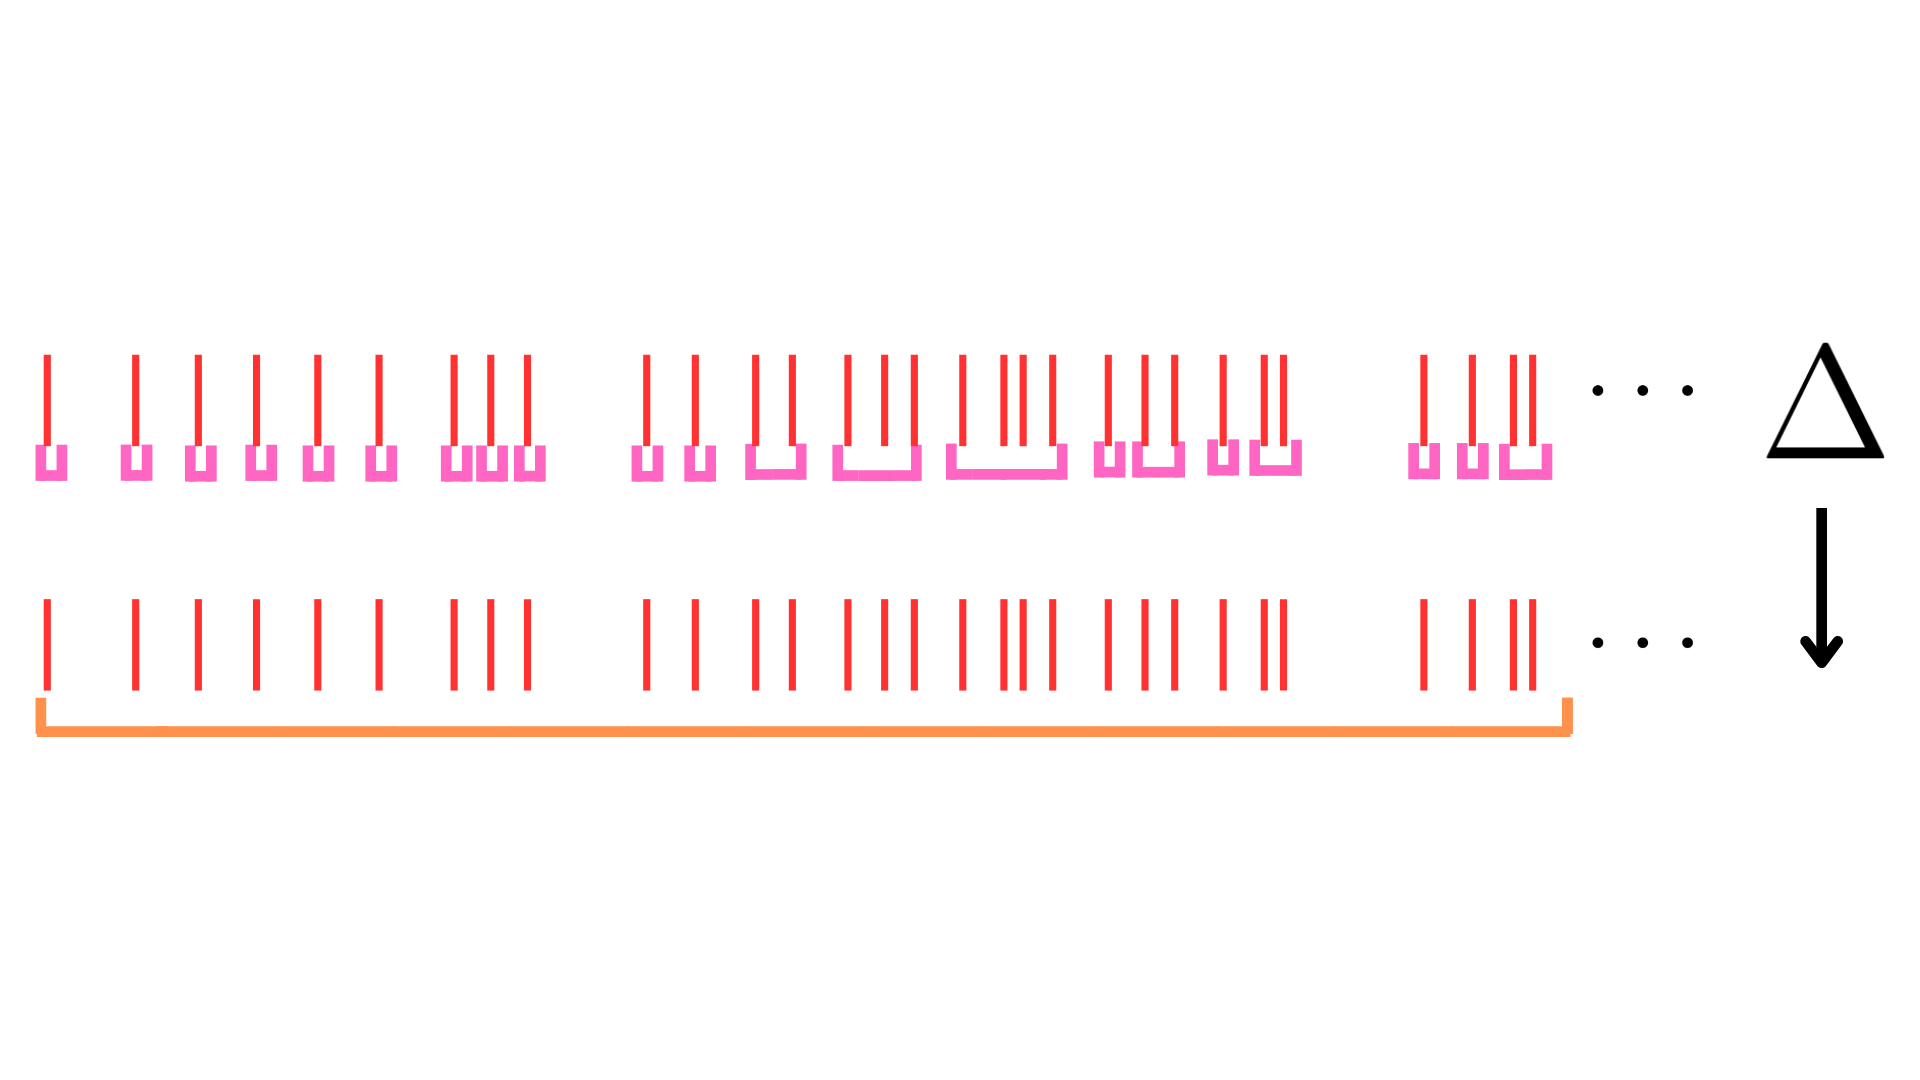
\includegraphics[width=0.9\textwidth]{Raster plot deltas 2.png}
    \caption{Diagram for $\mu\gg1$. Red lines represent the events, clusters are coloured. In this situation, events occur more regularly, resulting in a unique transition corresponding 
    the case of $\Delta$ is similar to the inter-event time producing the system percolation.}
    \label{f: Delta percolación 2}
\end{figure}
